\documentclass{beamer}
\usetheme{Warsaw}

\usepackage[utf8]{inputenc}
\usepackage{fancybox}
\usepackage{multimedia} 
\usepackage{subfig}
\usepackage{amsmath}

\usepackage[all]{xy}
\begin{document}


\title[Computergrafik] % (optional, only for long titles)
{Computergrafik

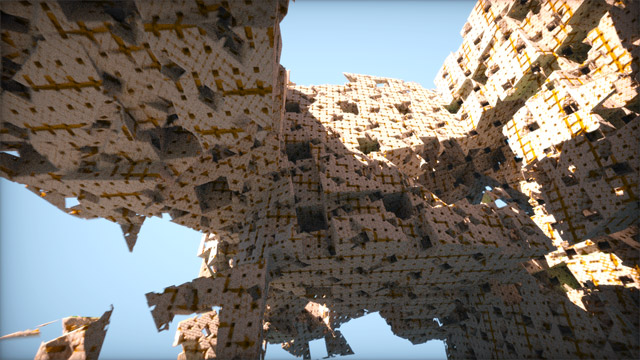
\includegraphics[scale=0.36]{images/cover}
}
\subtitle{}
\author[Dr. Johannes Riesterer] % (optional, for multiple authors)
{Dr.  rer. nat. Johannes Riesterer}

\date[KPT 2004] % (optional)
{}

\subject{Computergrafik}


\begin{frame}
    \frametitle{Computergrafik}
\framesubtitle{Echzeit Darstellung}
    \begin{block}{Echzeit Darstellung}
\begin{table}[h]
    \centering
    \begin{tabular}{|l|l|}
    \hline
    \textbf{Echtzeit-Typ} & \textbf{Eigenschaften} \\ \hline
    \textbf{Harte Echtzeit} & \begin{tabular}[c]{@{}l@{}}Zeitlimits zwingend, \\ Systemfehler bei Verpassen.\end{tabular} \\ \hline
    \textbf{Weiche Echtzeit} & \begin{tabular}[c]{@{}l@{}}Kleine Abweichungen erlaubt, \\ Leistung sinkt bei Überschreitung.\end{tabular} \\ \hline
    \end{tabular}
   % \caption{Definitionen von Echtzeitsystemen}
    \end{table}
    
\end{block}

\end{frame}


\begin{frame}
    \frametitle{Computergrafik}
\framesubtitle{Echzeit Darstellung}
    \begin{block}{Echzeit Darstellung}
Standard: $60$ Frames pro Sekunde bei einer Bildschirmauflösung von $4K=3840 \times 2160$ Pixel.  
D.h. $497.664.000$ Farbwerte müssen pro Sekunde berechnet und an das Ausgabegerät
geschickt werden. 
Kombination von Soft- und Hardware nötig.
\end{block}
\begin{table}[h]
    \centering
    \tiny % Schriftgröße ändern
    \begin{tabular}{|l|l|l|}
    \hline
    \textbf{GPU-Klasse} & \textbf{FP32-Leistung} & \textbf{FP64-Leistung} \\ \hline
    \textbf{Einsteiger- / Mittelklasse} & 2 - 10 TFLOPS & 0,1 - 1 TFLOPS \\ \hline
    \textbf{High-End-Gaming} & 10 - 25 TFLOPS & 0,5 - 2 TFLOPS \\ \hline
    \textbf{Workstation- / AI-GPUs} & 20 - 40 TFLOPS & 5 - 20 TFLOPS \\ \hline
    \textbf{Spezialisierte Hochleistung} & Mehrere 100 TFLOPS & Mehrere 20+ TFLOPS \\ \hline
    \end{tabular}
    \end{table}

\end{frame}




\begin{frame}{Aufbau und Funktionsweise einer GPU}
    \begin{itemize}
      \item \textbf{Architektur:} Viele einfache Rechenkerne in \textit{Streaming Multiprocessors (SM)}, optimiert für parallele Berechnung.
      \item \textbf{Speicherhierarchie:}
      \begin{itemize}
        \item \textit{Global Memory (VRAM)}: Großer, langsamer Speicher für die gesamte GPU.
        \item \textit{Shared Memory}: Schneller Zwischenspeicher pro SM.
        \item \textit{Register}: Klein, extrem schnell, lokal pro Kern.
      \end{itemize}
      \item \textbf{SIMD-Prinzip:} Gleiche Operation auf mehrere Daten gleichzeitig (Single Instruction, Multiple Data).
      \item \textbf{Thread-Modell:} Threads in \textit{Thread-Blocks} organisiert, diese in einem \textit{Grid}.
      \item \textbf{Spezialisierte Hardware:} Rasterisierung, Texturierung und Shading für Grafikoperationen.
    \end{itemize}
  \end{frame}



\begin{frame}
    \frametitle{Computergrafik}
\framesubtitle{}

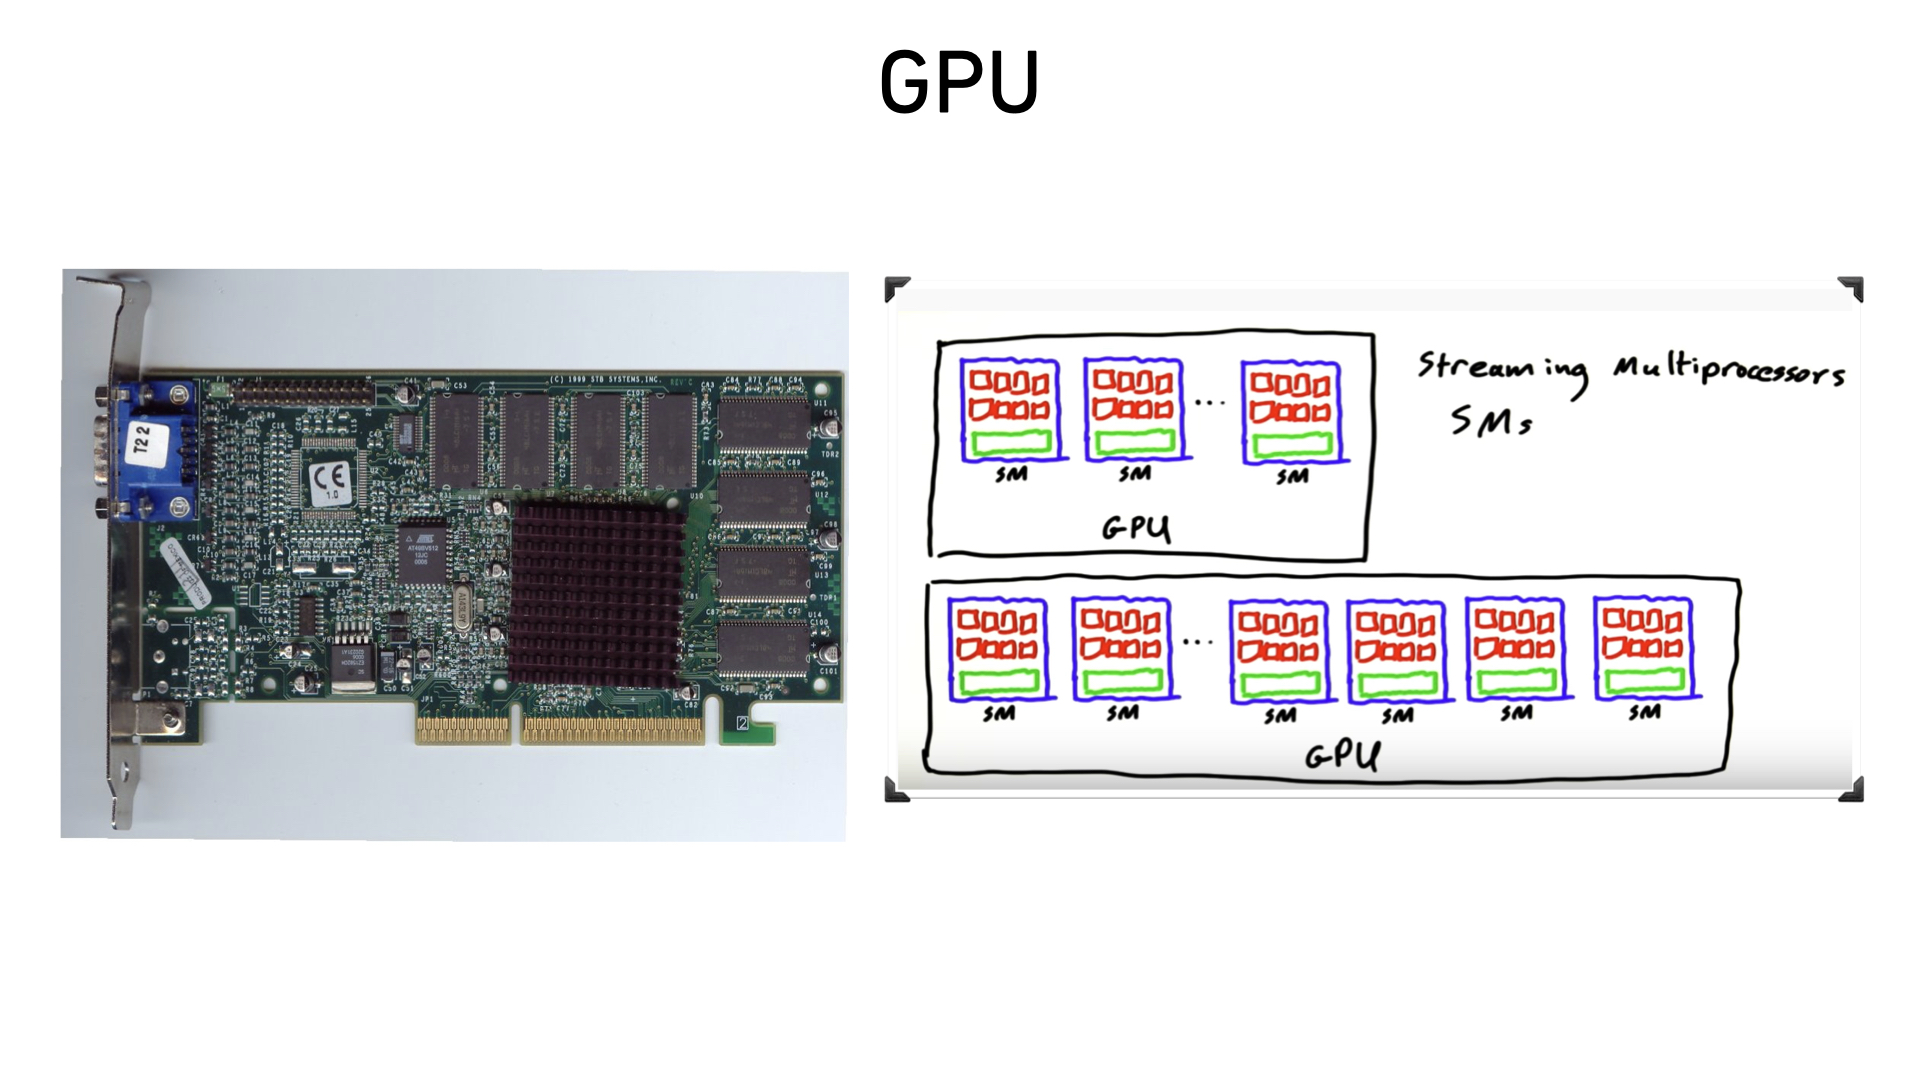
\includegraphics[scale=0.16]{images/Shaderday_Intro/Shaderday_Intro_004} \\
\end{frame}

\begin{frame}
    \frametitle{Computergrafik}
\framesubtitle{}

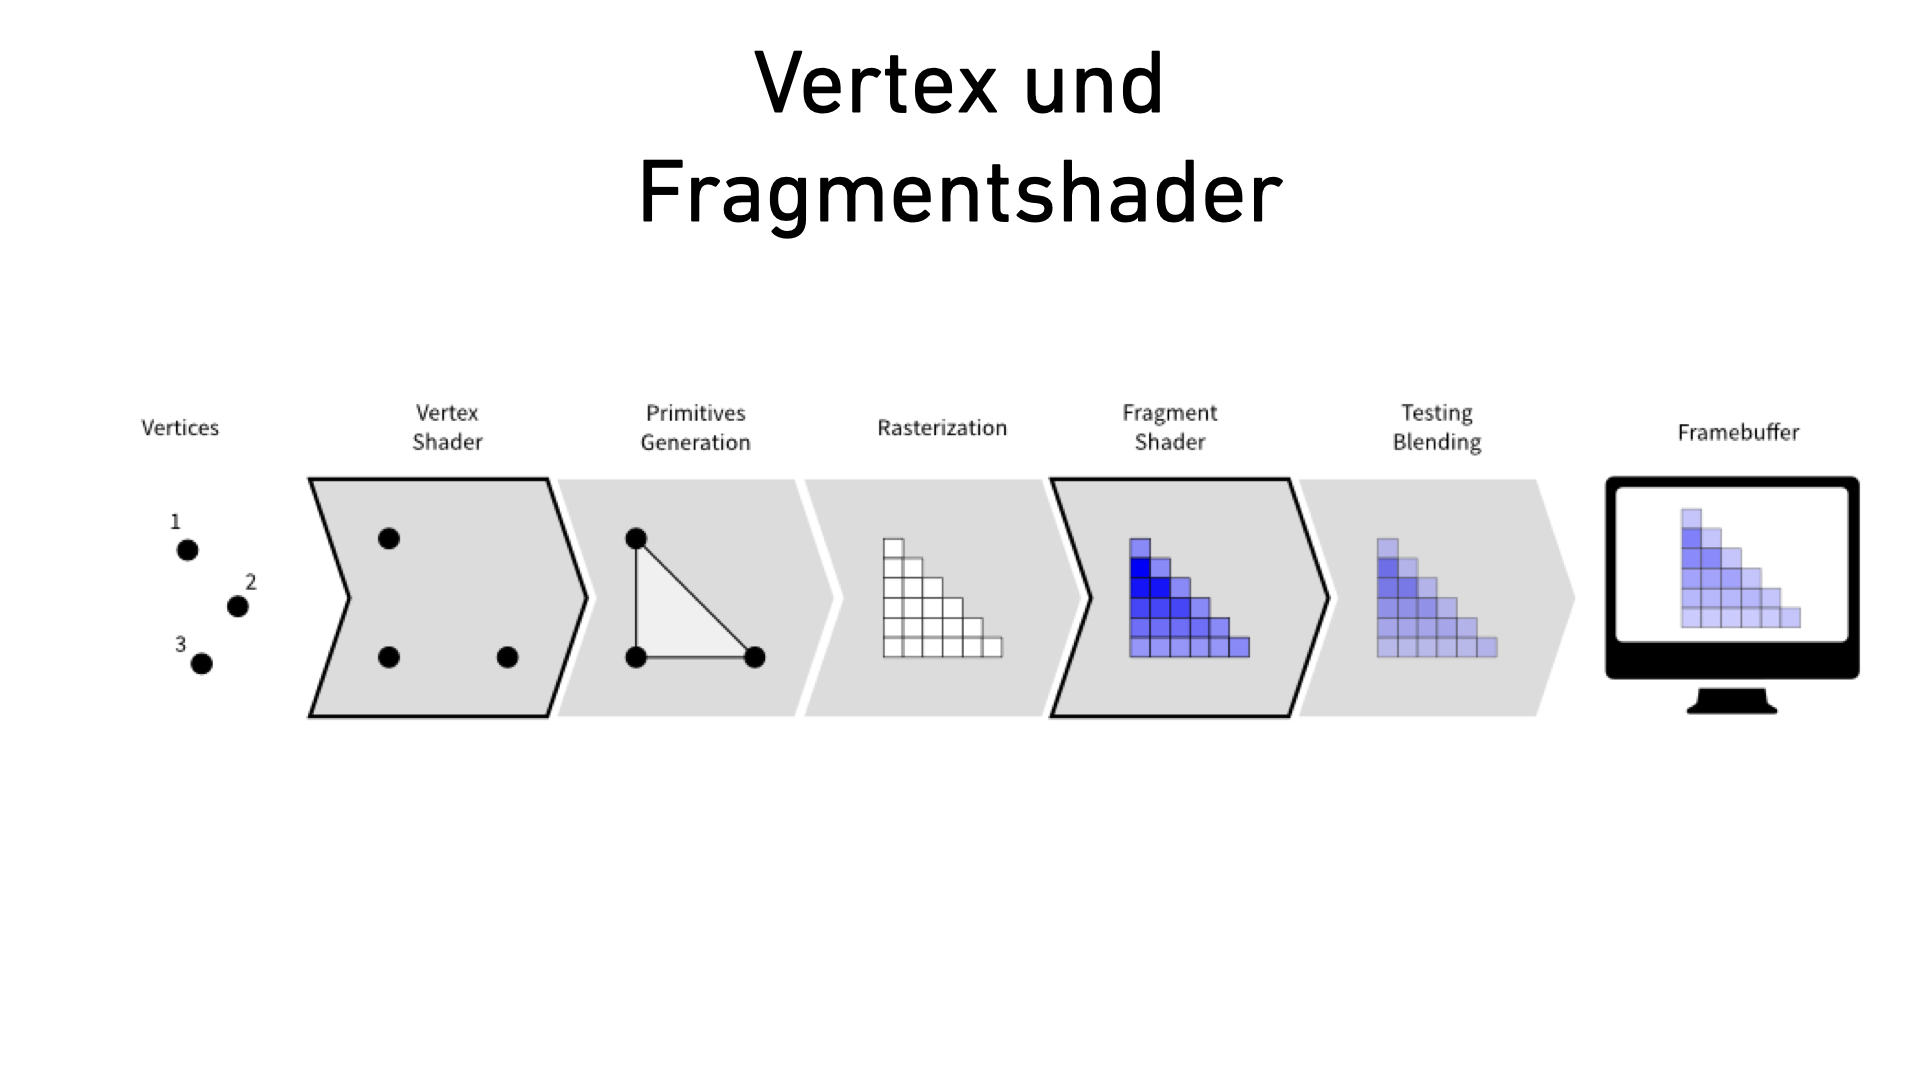
\includegraphics[scale=0.15]{images/Shaderday_Intro/Shaderday_Intro_007}

\end{frame}


\begin{frame}
    \frametitle{Computergrafik}
\framesubtitle{}

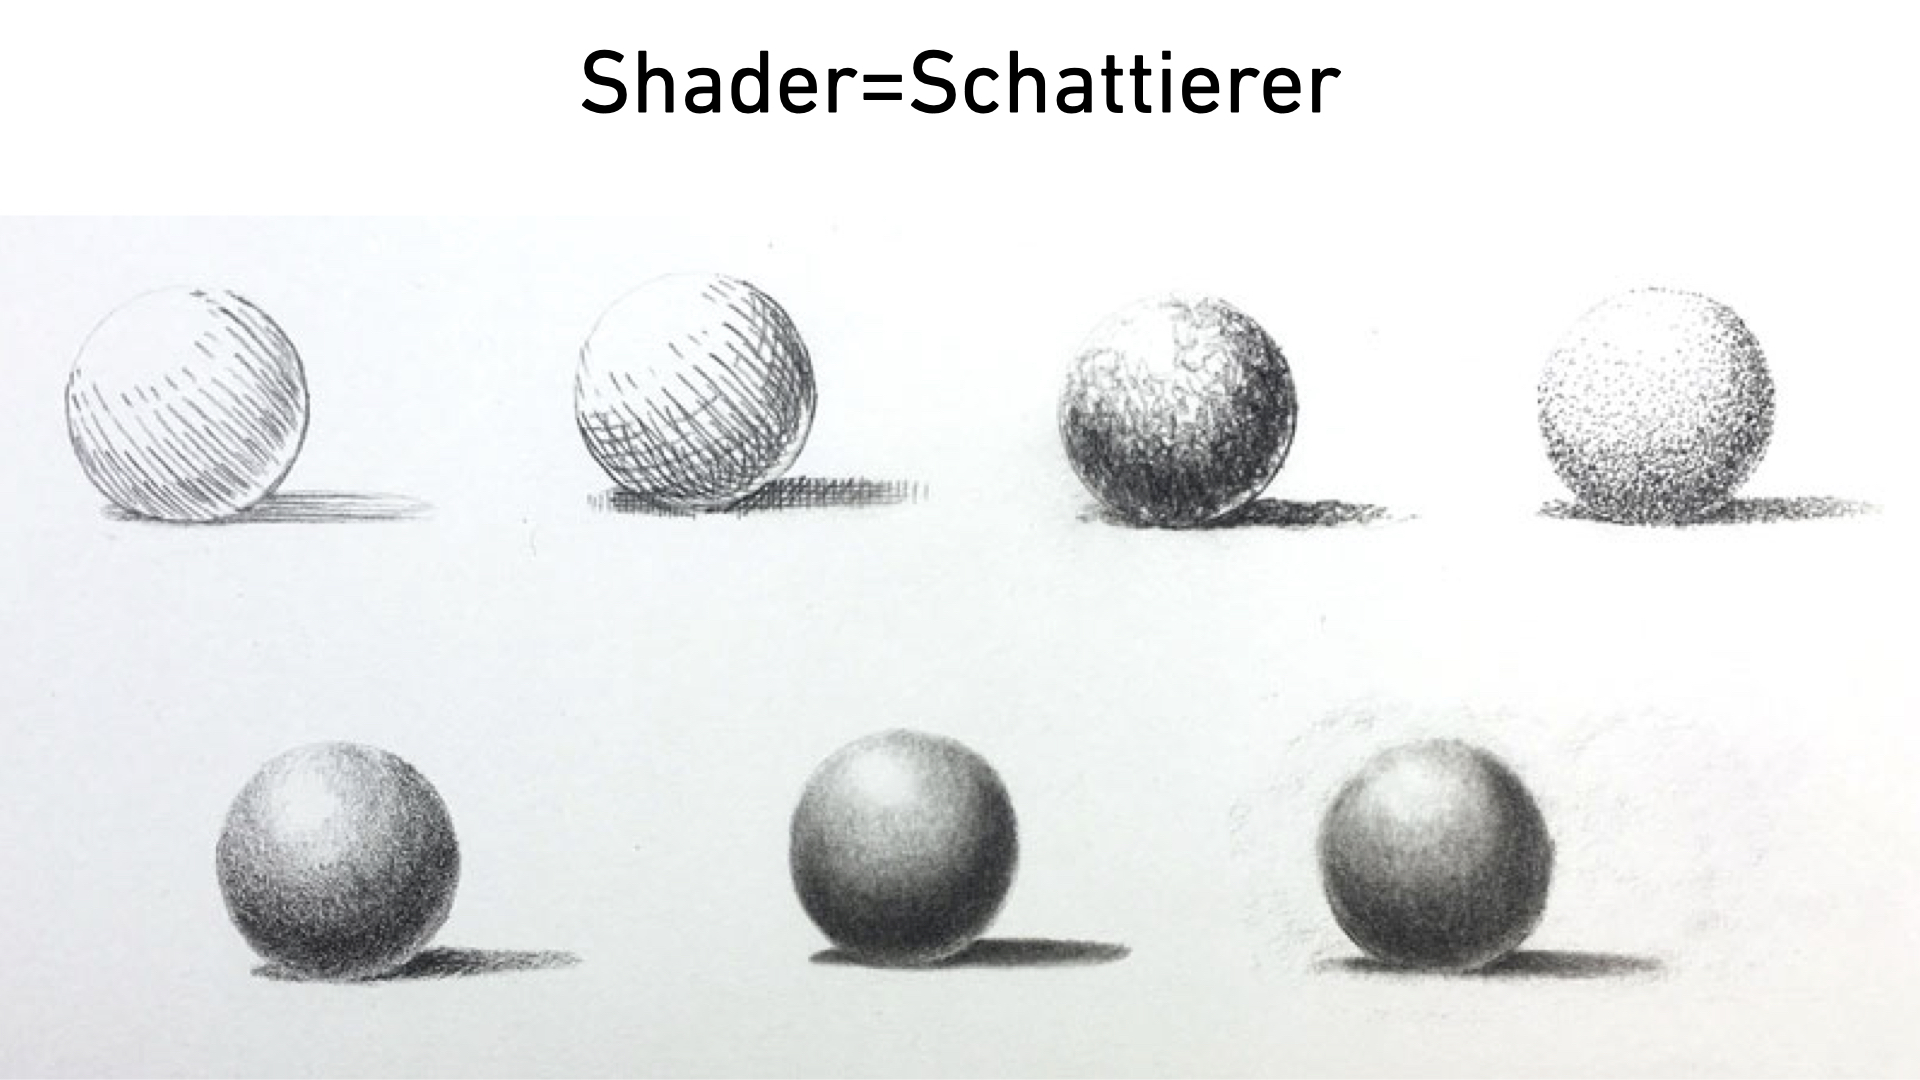
\includegraphics[scale=0.15]{images/Shaderday_Intro/Shaderday_Intro_001} 
\end{frame}



  
\begin{frame}
    \frametitle{ Shaderprogramm}
\framesubtitle{}
\begin{center}
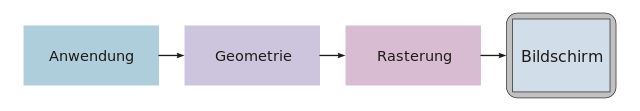
\includegraphics[scale=0.26]{images/cgpipeline_grob}
\\
\includegraphics[scale=0.20]{images/Zeichnung_Shaderpipeline}

\end{center}
\end{frame}

\begin{frame}
    \frametitle{OpenGL Pipeline}
\framesubtitle{}
    \begin{block}{}
\begin{center}
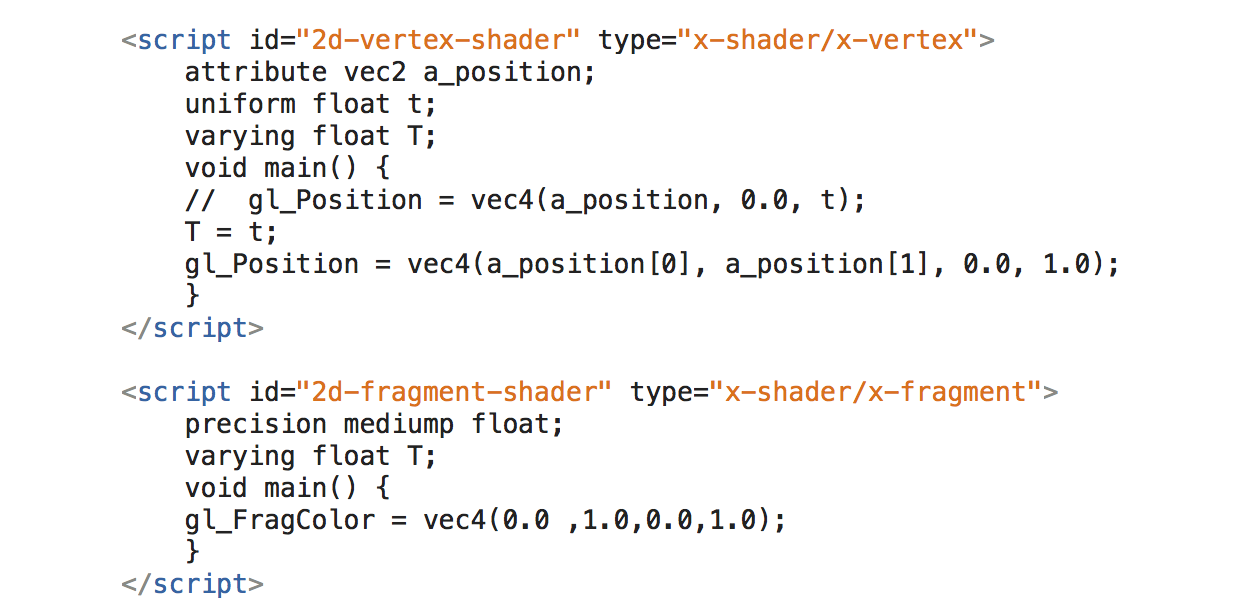
\includegraphics[scale=0.56]{images/shader}
\end{center}
\end{block}
\end{frame}


  
  \begin{frame}{Echzeit Darstellung}
    \begin{block}{Animation}
   Bewegungsabläufe werden durch eine Abfolge von statischen Bildern erzeugt, die so schnell nacheinander angezeigt werden, dass im Gehirn der Eindruck einer kontinuierlichen Bewegung entsteht. 
    Diese Abfolge von Bildern wird als Frames bezeichnet. 
    Die Illusion einer flüssigen Bewegung wird durch ein Phänomen in unserem visuellen System erzeugt, das als "Bewegungs-Nachbilder" oder auch "Persistence of Vision" bekannt ist.
\end{block}
\end{frame}
  

\begin{frame}{Begriff der Animation}
    \begin{itemize}
      \item \textbf{Illusion im Gehirn:}
      \begin{itemize}
        \item \textbf{Nachbilder im Auge:} Bilder verbleiben kurzzeitig auf der Netzhaut (ca. 1/25 Sekunde).
        \item \textbf{Verarbeitung im Gehirn:} 
        \begin{itemize}
          \item Aufeinanderfolgende Bilder werden kombiniert.
          \item Übergänge werden als kontinuierliche Bewegung interpretiert.
        \end{itemize} 
        \item \textbf{Bewegungswahrnehmung:} Spezialisierte Neuronen erkennen Bildunterschiede als Bewegung.
      \end{itemize}
      \item \textbf{Bildrate (Frames per Second, FPS):}
      \begin{itemize}
        \item \textbf{Unter 12 FPS:} Einzelbilder werden als ruckartig wahrgenommen.
        \item \textbf{Ab 24 FPS:} Flüssige Bewegung, typisch für Filme.
        \item \textbf{60 FPS:} Realistische Darstellung, z.B. in Computerspielen.
      \end{itemize}
    \end{itemize}
  \end{frame}
  

  \begin{frame}
    \frametitle{Echtzeit}
\framesubtitle{}
    \begin{block}{Chronofotografie}
        Die Chronofotografie (auch Fotochronografie) bezeichnet die fotografische Dokumentation von Bewegungen oder Prozessen, heute hauptsächlich als Hochgeschwindigkeitsfotografie. 
\end{block}

\begin{block}{Chronofotografie}
    In der Entwicklung der Fotografie wurden in den 1870er und 1880er Jahren durch empfindliche Photomaterialien und schnelle Kameraverschlüsse sogenannte Augenblicks- oder Momentfotografien möglich, Aufnahmen bewegter Objekte.
\end{block}
\end{frame}


\begin{frame}
    \frametitle{Computergrafik}
\framesubtitle{}
    \begin{block}{Chronofotografie}
        Muybridge gelang 1878 der Nachweis, dass ein Pferd im Galopp kurzzeitig mit allen vier Hufen vom Boden abhebt. Diese frühen Serienaufnahmen lieferten wichtige Impulse für die Entwicklung der bewegten Bilder und waren damit auch Vorläufer des Kinofilms. 
    \end{block}
    \begin{center}
        
        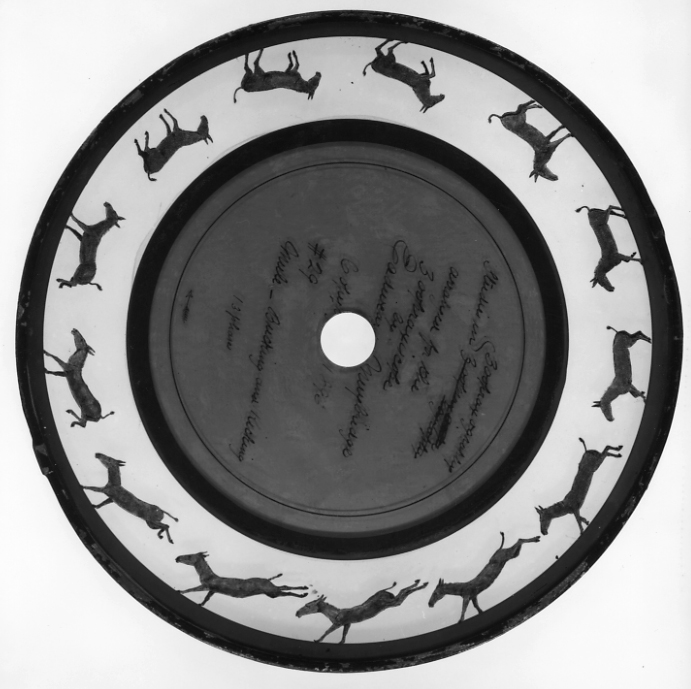
\includegraphics[scale=0.36]{images/Zoopraxiscope.jpg}
    \end{center}
   
\end{frame}


\end{document}
